\documentclass[twoside]{scrarticle}
\let\tempmargin\oddsidemargin
\let\oddsidemargin\evensidemargin
\let\evensidemargin\tempmargin
\reversemarginpar

\usepackage{graphicx, float, caption}
\usepackage{amsmath} 
\begin{document}
	\title{Tugas KPB Bab 13}
	\author{Muhamad Risqi Aditiya \protect\\ 5024221010}
	
	\maketitle
	
	\section*{Soal}
	\begin{enumerate}
		\item[23. ]
		Diketahui : $x = t,\;y = \frac{1}{1 + t^2},\;z = t^2$
		
		Ditanya : Cocokkan persamaan parametrik dengan grafik (I-VI) !
		
		Jawab : Semua bilangan real memenuhi persamaan, sehingga didapat grafik sebagai berikut
		
		\begin{minipage}{\linewidth}
			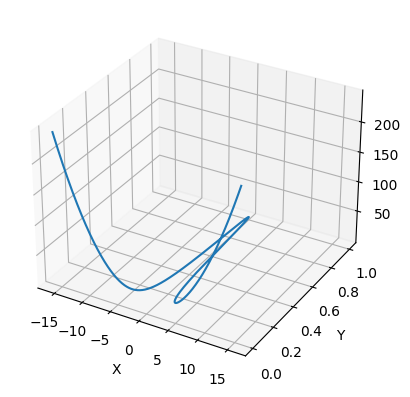
\includegraphics[width=0.5\textwidth]{image2.png}
			\centering
			\captionof{figure}{No. 23}
		\end{minipage}
		
		Menurut visualisasi, persamaan cocok dengan grafik no VI
		
		\item[27.] Diketahui : Persamaan parametrik $x =
		t\;cos\;t,y=t\;sin\;t, z=t$ ,dan kerucut $z^2 = x^2 + y^2$
		
		Ditanya : Tunjukkan persamaan parametrik tersebut memenuhi persamaan kerucut tersebut, dan gunakan data diatas untuk membantu membuat sketsa grafik!
		
		Jawab : Berdasarkan data yang ada, didapatkan garfik berikut ini
		
		\begin{minipage}{\linewidth}
			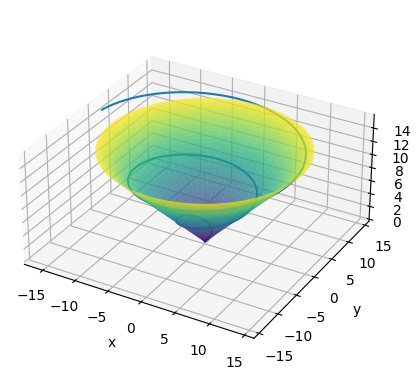
\includegraphics[width=0.5\textwidth]{27.png}
			\centering
			\captionof{figure}{No. 27}
		\end{minipage}
		
		Sehingga berdasarkan grafik diatas kita dapat bahwa persamaan parametrik berada pada permukaan kerucut. Itu artinya BENAR bahwa persamaan parametrik tersebut memenuhi persamaan kerucut tersebut
		
		\item[31.] Diketahui : $r(t) = <cos\;t\;sin\;2t, sin\;tsin\;2t, cos\;2t>$
		
		Ditanya : Buatlah grafik menggunakan komputer berdasarkan persamaan yang diberikan !
		
		Jawab: Semua domainnya bilangan real, sehingga didapat grafik sebagai berikut
		
		\begin{minipage}{\linewidth}
			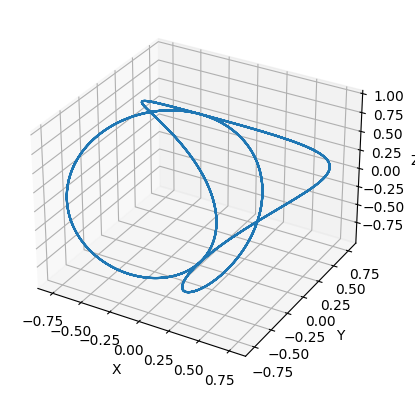
\includegraphics[width=0.5\textwidth]{31.png}
			\centering
			\captionof{figure}{No. 31}
		\end{minipage}
		
		\item[32.] Diketahui : $r(t) = <t^2, ln\;t, t>$
		
		Ditanya : Buatlah grafik menggunakan komputer berdasarkan persamaan yang diberikan !
		
		Jawab: Karena terdapat $ln\;t$ dimana t tidak boleh negatif maka domainnya adalah $t > 0$, sehingga didapat grafik sebagai berikut
		
		\begin{minipage}{\linewidth}
			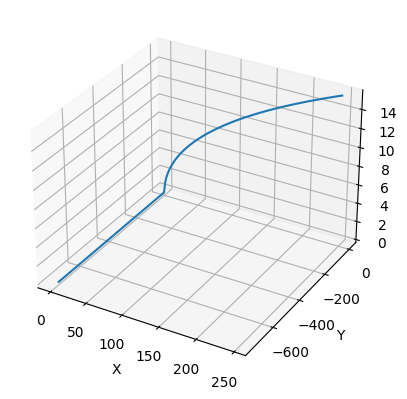
\includegraphics[width=0.5\textwidth]{32.png}
			\centering
			\captionof{figure}{No. 32}
		\end{minipage}
		\item[33.] Diketahui : $r(t) = <t, t\;sin\;t, t\;cos\;t> $
		
		Ditanya : Buatlah grafik menggunakan komputer berdasarkan persamaan yang diberikan !
		
		Jawab: Semua bilangan real memenuhi persamaan, sehingga didapat grafik sebagai berikut
		
		\begin{minipage}{\linewidth}
			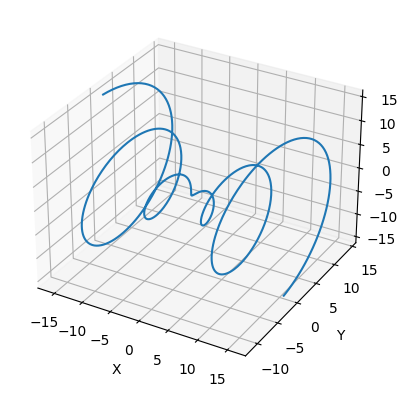
\includegraphics[width=0.5\textwidth]{33.png}
			\centering
			\captionof{figure}{No. 33}
		\end{minipage}
		
		\item[34.] Diketahui : $r(t) = <t, e^t, cos\;t> $
		
		Ditanya : Buatlah grafik menggunakan komputer berdasarkan persamaan yang diberikan !
		
		Jawab: Semua bilangan real memenuhi persamaan, sehingga didapat grafik sebagai berikut
		
		\begin{minipage}{\linewidth}
			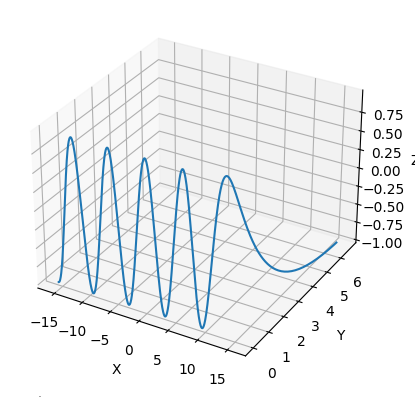
\includegraphics[width=0.5\textwidth]{34.png}
			\centering
			\captionof{figure}{No. 34}
		\end{minipage}
		
		\item[35.] Diketahui : $r(t) = <cos\;2t, cos\;3t, cos\;4t> $  
		
		Ditanya : Buatlah grafik menggunakan komputer berdasarkan persamaan yang diberikan !
		
		Jawab: Semua bilangan real memenuhi persamaan, sehingga didapat grafik sebagai berikut
		
		\begin{minipage}{\linewidth}
			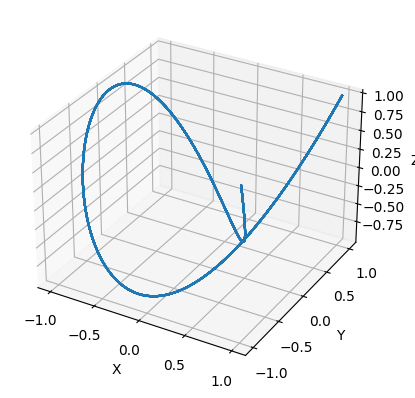
\includegraphics[width=0.5\textwidth]{35.png}
			\centering
			\captionof{figure}{No. 35}
		\end{minipage}
		
		\item[36.] Diketahui : persamaan parametrik $x = sin\;t, y = sin\;2t, z = cos\;3t$.
		
		Ditanya : Sketsakan kurva parametrik tersebut, dan jelaskan bentuknya dengan membuat grafik proyeksinya pada tiga bidang koordinat.
		
		Jawab : Berikut merupakah grafik dari persamaan diatas dalam bidang 3 koordinat
		
		\begin{minipage}{\linewidth}
			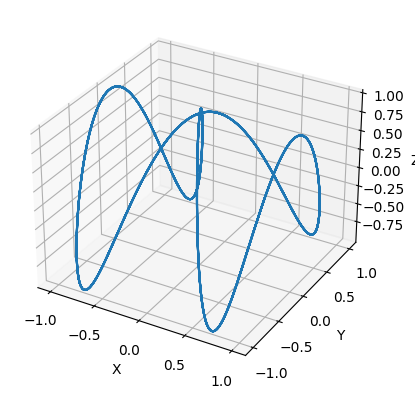
\includegraphics[width=0.5\textwidth]{36.png}
			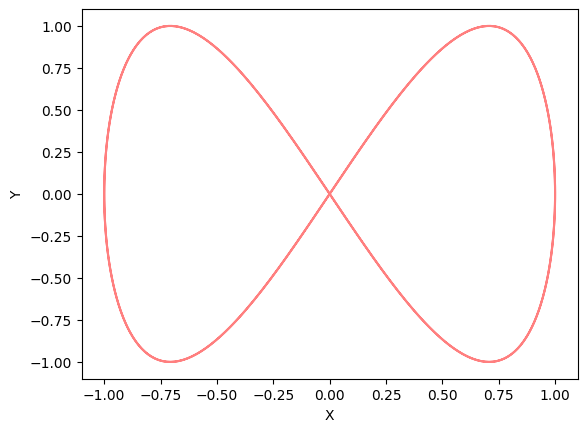
\includegraphics[width=0.5\textwidth]{36_xy.png}
			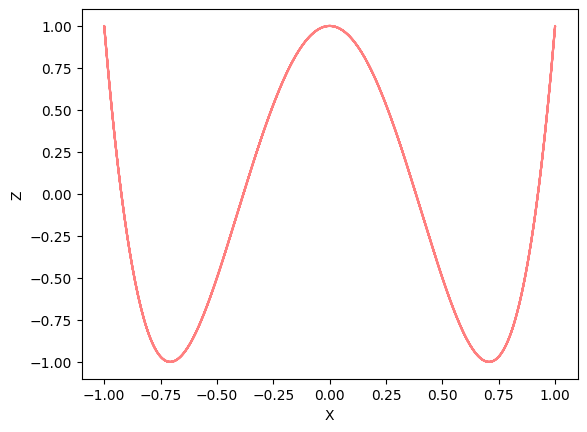
\includegraphics[width=0.5\textwidth]{36_xz.png}
			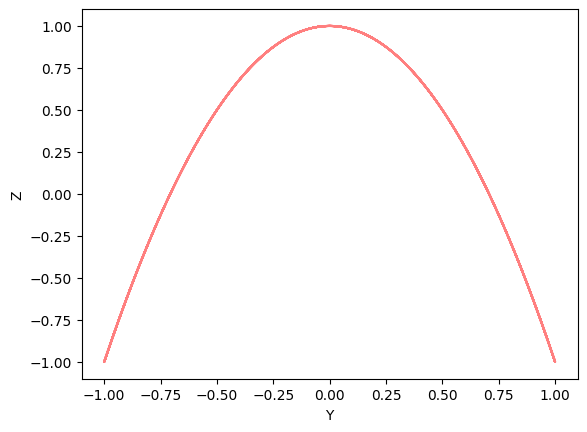
\includegraphics[width=0.5\textwidth]{36_yz.png}
			\captionof{figure}{No. 36}
		\end{minipage}
		
		Berdasarkan gambar tersebut, didapatkan bahwa semua bilangan real memenuhi persamaan. 
		
		\item[37.] Diketahui : persamaan parametrik sebagai berikut
		\begin{equation*}
			\begin{aligned}
				x & = (1+cos\;16t)\;cos\;t\\
				y & = (1+cos\;16t)\;sin\;t\\
				z & = 1 + cos\;16t
			\end{aligned}
		\end{equation*}
		
		Ditanya : Buatlah grafik kurva dengan persamaan parametrik diatas, lalu jelaskan kenampakan grafik dengan menunjukkan grafik terletak pada kerucut !
		
		Jawab: Berikut merupakan sketsa grafiknya
		
		\begin{minipage}{\linewidth}
			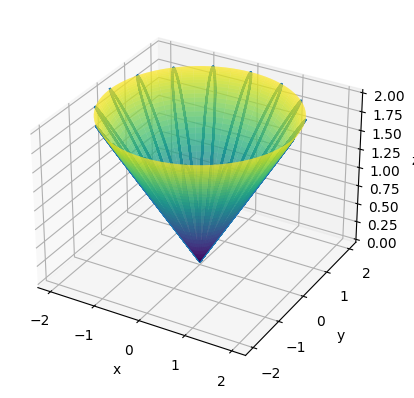
\includegraphics[width=0.5\textwidth]{37.png}
			\centering
			\captionof{figure}{No. 37}
		\end{minipage}
		
		Semua bilangan real memenuhi persamaan, lalu didapat bahwa persamaan parametrik tersebut terlihat seperti memliki semacam gelombang pada permukaan kerucut.
		
		\item[38.] Diketahui : persamaan parametrik sebagai berikut
		\begin{equation*}
			\begin{aligned}
				x & = \sqrt{1-0.25\;cos^2t}\;cos\;t\\
				y & = \sqrt{1-0.25\;cos^2t}\;sin\;t\\
				z & = 0.5\;cos\;10t
			\end{aligned}
		\end{equation*}
		
		Ditanya : Buatlah grafik kurva dengan persamaan parametrik diatas, lalu jelaskan kenampakan grafik dengan menunjukkan grafik terletak pada kerucut !
		
		Jawab: Berikut merupakan sketsa grafiknya
		
		\begin{minipage}{\linewidth}
			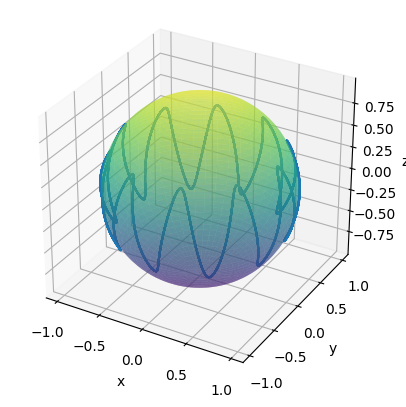
\includegraphics[width=0.5\textwidth]{38.png}
			\centering
			\captionof{figure}{No. 38}
		\end{minipage}
		
		Semua bilangan real memenuhi persamaan, lalu didapat juga seperti gelombang pada permukaan bola sama seperti kenampakan gelombang pada grafik no. 37. Bola didapat dengan plotting
		Bola dengan pusat (0, 0) dan jari jari 1
		
		\item[41.] Diketahui : Kerucut $z = \sqrt{x^2 + y^2}$ ,and Bidang $z = 1+y$
		
		Ditanya : Tentukan fungsi vektor yang menyatakan kurva perpotongan kedua permukaan !
		
		Jawab: Berdasarkan data diatas didapat grafik sebagai berikut
		
		\begin{minipage}{\linewidth}
			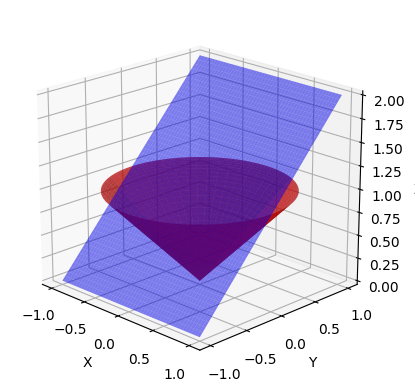
\includegraphics[width=0.5\textwidth]{41.png}
			\centering
			\captionof{figure}{No. 41}
		\end{minipage}
		
		Dari grafik tersebut ditemukan bahwa semua bilangan real memenuhi persamaan, dan didapatkan juga bahwa bidang $z = 1 + y$ memotong kerucut $z = \sqrt{x^2 + y^2}$ 
		
		\item[45.] Diketahui : selinder $x^2 + y^2=4$, dan selinder parabola  $z = x^2$
		
		Ditanya : Buatlah sketsa grafik selinder diatas, lalu temukan persamaan parametrik untuk kurva yang berpotongan tersebut lalu sketsakan !
		
		Jawab: Semua bilangan real memenuhi persamaan, lalu didapat persamaan parametriknya sebagai berikut
		\begin{equation*}
			\begin{aligned}
				x^2 + y^2 & = 4\\
				z & = x^2\\
			\end{aligned}
		\end{equation*}
		\centerline{maka}
		\begin{equation*}
			\begin{aligned}
				x & =2\;cos\;t\\
				y & =2\;sin\;t\\
				z & = x^2\\
				& = (2\;cos\;t)^2\\
				& = 4\;cos^2\;t\\ 
			\end{aligned}
		\end{equation*}
		
		Maka dengan begitu didapat sketsa grafik slindernya dan grafik kurva perpotongannya seperti dibawah ini
		
		\begin{minipage}{\linewidth}
			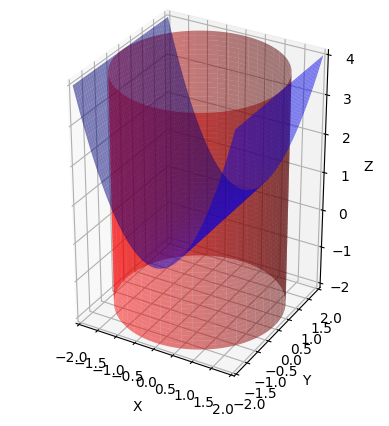
\includegraphics[width=0.5\textwidth]{45.png}
			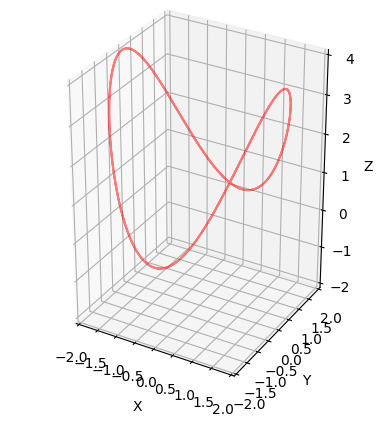
\includegraphics[width=0.5\textwidth]{45_1.png}
			\captionof{figure}{No. 45}
		\end{minipage}
		
		\item[46.] Diketahui : Selinder parabola $y=x^2$, dan separuh atas ellipsoid $x^2+4 y^2+4 z^2=16$
		
		Ditanya : Buatlah sketsa grafik selinder diatas, lalu temukan persamaan parametrik untuk kurva yang berpotongan tersebut lalu sketsakan !
		
		Jawab: Semua bilangan real memenuhi persamaan, lalu didapat persamaan parametriknya sebagai berikut
		\begin{equation*}
			\begin{aligned}
				y & = x^2\\
				x^2 + 4 y^2 + 4 z^2 & = 16\\
			\end{aligned}
		\end{equation*}
		\centerline{maka}
		\begin{equation*}
			\begin{aligned}
				x & = t\\
				y & = t^2\\
				4z^2 & = 16 - x^2 - 4y^2\\
				z^2 & = 4 - \frac{x^2}{4} - y^2\\
				z & = \sqrt{4 - \frac{x^2}{4} - y^2}\\
				z & = \sqrt{4 - \frac{t^2}{4} - t^4}\\
			\end{aligned}
		\end{equation*}
		
		Maka dengan begitu didapat sketsa grafik slindernya dan grafik kurva perpotongannya seperti dibawah ini
		
		\begin{minipage}{\linewidth}
			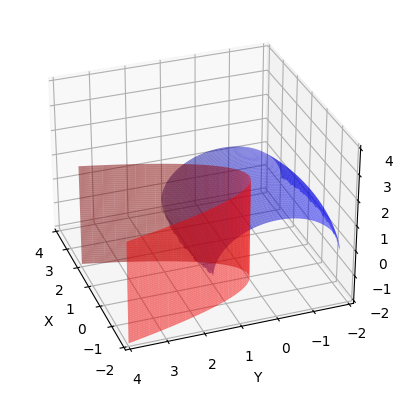
\includegraphics[width=0.5\textwidth]{46.png}
			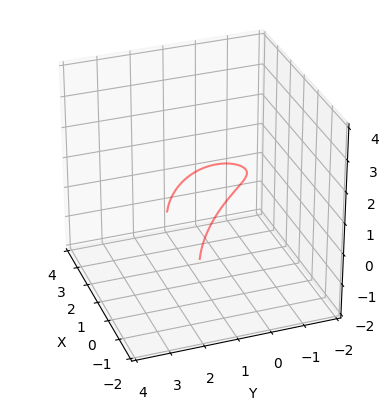
\includegraphics[width=0.5\textwidth]{46_1.png}
			\captionof{figure}{No. 46}
		\end{minipage}
		
		\item[50.] Diketahui : persamaan parametrik sebagai berikut
		\begin{equation*}
			\begin{aligned}
				& x=(2+\cos 1.5 t) \cos t \\
				& y=(2+\cos 1.5 t) \sin t \\
				& z=\sin 1.5 t
			\end{aligned}
		\end{equation*}
		untuk membuat sketsa kurva dengan tangan seperti yang dilihat dari atas, dengan celah yang menunjukkan di mana kurva melewatinya. Mulailah dengan menunjukkan itu proyeksi kurva ke bidang $x y$ memiliki koordinat kutub $r=2+\cos 1.5 t$ dan $\theta=t$, jadi $r$ bervariasi antara 1 dan 3. Kemudian tunjukkan bahwa $z$ memiliki nilai maksimum dan minimum ketika proyeksi berada di tengah-tengah antara $r=1$ dan $r=3$.
		
		Ditanya : Sketsakan kurva dengan sudut pandang tepat di atas, kemudian sketsakan kurva dari beberapa sudut pandang lainnya untuk mendapatkan kesan yang lebih baik ! 
		
		Jawab: Semua bilangan real memenuhi persamaan. Grafik dan proyeksinya terhadap ke tiga bidang adalah sebagai beriikut
		
		\begin{minipage}{\linewidth}, 
			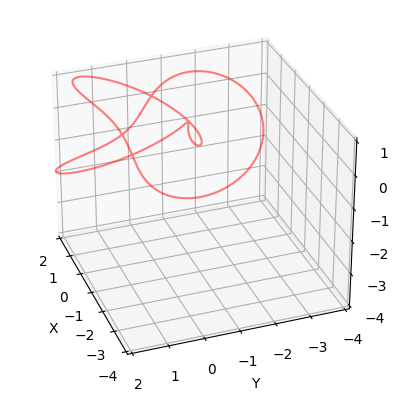
\includegraphics[width=0.5\textwidth]{50.png}
			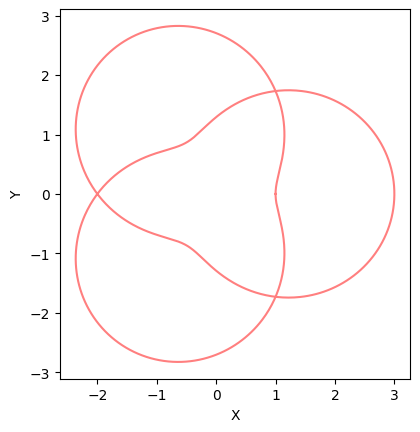
\includegraphics[width=0.5\textwidth]{50_1.png}
			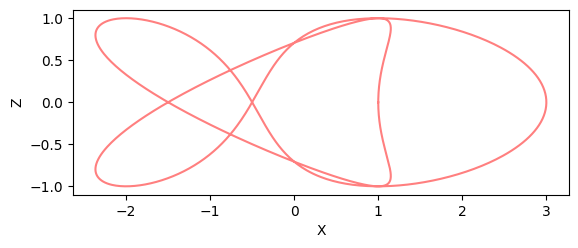
\includegraphics[width=0.5\textwidth]{50_2.png}
			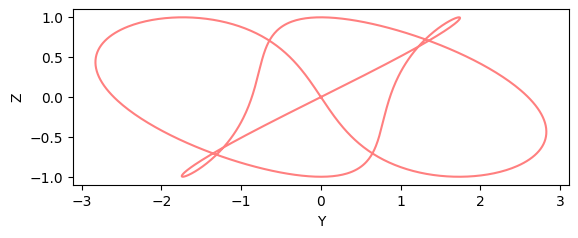
\includegraphics[width=0.5\textwidth]{50_3.png}
			\captionof{figure}{No. 50} 
		\end{minipage}
		
		Berdasarkan keempat grafik diatas, didapat bahwa proyeksi pada bidang $xy$ lebih menunjukkan bentuk sebenarnya dari fungsi parametrik tersebut.
		
	\end{enumerate}
\end{document}